% !TEX program = latexmk
% !TEX encoding = UTF-8 Unicode
\documentclass[varwidth=\maxdimen]{standalone}

\usepackage{expl3}
\usepackage{ifxetex}
\RequireXeTeX

%%% tikz %%%
\usepackage{tikz}
\usepackage{tikz-3dplot}
\usepackage{pgfplots}
\usetikzlibrary{
  shapes,
  arrows,
  positioning,
  calc,
  graphs,
  intersections,
  circuits.ee.IEC,
  quotes,
  shapes.geometric,
}

\newlength\tikzboxwidth
\newlength\tikzboxheight
\newcommand\tikzbox[1]{%
  \settowidth\tikzboxwidth{#1}%
  \settoheight\tikzboxheight{#1}%
  \begin{tikzpicture}
  \path[use as bounding box]
    (-0.5\tikzboxwidth,-0.5\tikzboxheight)rectangle
    (0.5\tikzboxwidth,0.5\tikzboxheight);
  \node[inner sep=\tabcolsep+0.5\arrayrulewidth,line width=0.5mm,draw=black]
    at(0,0){#1};
  \end{tikzpicture}%
}


\usepackage[tbtags]{amsmath}
\usepackage{unicode-math}
\usepackage{amsthm}
\usepackage{lmodern}
\usepackage{anyfontsize}
\usepackage{mathrsfs}
\usepackage{amsfonts}


\usepackage{xeCJK}
\usepackage[T1]{fontenc}
\setCJKmainfont[AutoFakeBold=true]{FandolSong}
\setmainfont{Times New Roman}
\setmathfont{XITS Math}
\newfontfamily{\ipa}{Doulos SIL}


\usepackage{ninecolors}
\usepackage{tabularray}
\NewTblrTheme{nocaption}{
    \DefTblrTemplate{caption}{default}{}
    \DefTblrTemplate{capcont}{default}{}
}

\begin{document}
\begin{talltblr}[
  theme=nocaption,
  note{*}={Symbols to the right in a cell are voiced, to the left are voiceless. Shaded areas denote articulations judged impossible.}
]{
  colspec={lcccccccccccccccccccccc},
  cell{2-Z}{2-Z}={font=\ipa\fontsize{12pt}{12pt}\selectfont},
  vline{even[2-6]},
  vline{even[12-Z]},
  vline{1},
  cell{1}{even[2-Y]}={c=2}{c},
  hlines,
  cell{2}{X,Z}={}{gray9},
  cell{7,9}{2-5}={}{gray9},
  cell{4,5}{16-17}={}{gray9},
  cell{3,7,9}{20-21}={}{gray9},
  cell{3-5,7-9}{22-23}={}{gray9},
  column{2-Z}={wd=2em,c},
  columns={colsep=1pt},
  vline{8,10}={1,6}{solid,black},
  vline{8,10}={2-5,7-9}{solid,gray6},
  vline{odd[3-Z]}={dashed,gray6},
}
& Bilabial & & Labiodental & & Dental & &  Alveolar & & Postalveolar & & Retroflex & & Palatal & & Velar & & Uvular & & Pharyngeal & & Glottal \\
Plosive & p & b & & & & & t & d & & & ʈ & ɖ & c & ɟ & k & g & q & ɢ & & & ʔ & \\
Nasal   & & m & ɱ & & & & n & & & & ɳ & & ɲ & & ŋ & & ɴ & & & & & \\
Trill   & & ʙ & & & & & & r & & & & & & & & & & ʀ & & & & \\
Tap or Flap & & & & ⱱ & & & & ɾ & & & & ɽ & & & & & & & & & & \\
Fricative & ɸ & β & f & v & θ & ð & s & z & ʃ & ʒ & ʂ & ʐ & ç & ʝ & x & ɣ & χ & ʁ & ħ & ʕ & h & ɦ \\
Lateral fricative & & & & & & & ɬ & ɮ & & & & & & & & & & & & & & \\
Approximant & & & & ʋ & & & & ɹ & & & & ɻ & & j & & ɰ & & & & & & \\
Lateral appoximant & & & & & & & & l & & & & ɭ & & ʎ & & ʟ & & & & & & \\
\end{talltblr}


\begin{talltblr}[
  theme=nocaption,
]{
  colspec={clclcl},
  cell{1}{odd[1-Z]}={c=2}{c},
  vline{odd},
  hline{1,2,Z},
  cell{2-Z}{1,3,5}={font=\ipa\fontsize{14pt}{14pt}\selectfont},
}
  Clicks & & Voiced implosives & & Ejectives & \\
  ʘ & Bilabial & ɓ & Bilabial & ◌ʼ & Examples: \\
  | & Dental & ɗ & Dental / alveolar & pʼ & Bilabial \\
  ! & (Post)alveolar & ʄ & Palatal & tʼ & Dental/alveolar \\
  ǂ & Palatoalveolar & ɠ & Velar & kʼ & Velar \\
  ǁ & Alveolar lateral & ʛ & Uvular & sʼ & Alveolar fricative \\
\end{talltblr}
\framebox{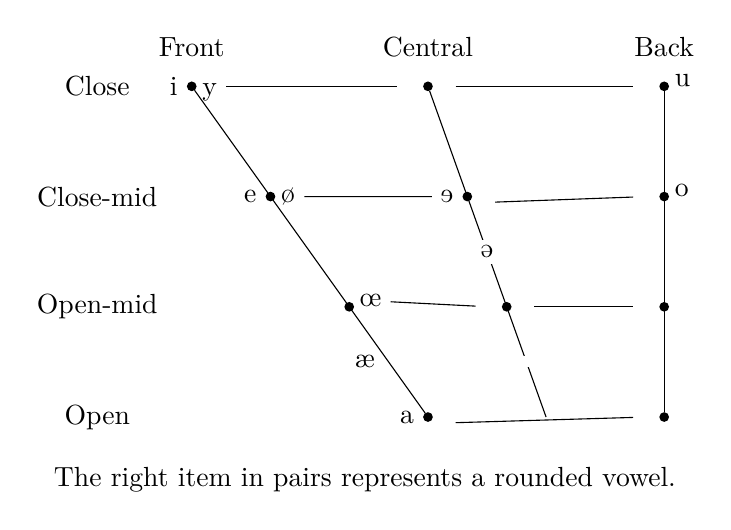
\begin{tikzpicture}[
  every node/.style={align=center, font=\fontsize{14pt}{14pt}\ipa, outer sep=0},
  node distance=0.25cm,
  align = center,
  dot/.style = {circle, fill, minimum size=#1,
              inner sep=0pt, outer sep=0pt},
  dot/.default = 3.5pt,
  baseline=(current bounding box.west)
]

\begin{scope}[xshift=0cm, yshift=0cm]
  \node [name=FC, dot] at (0, 0) {}; \node [left=0pt of FC, name=FC-L] {i}; \node[right, base right=2.3pt of FC-L, name=FC-R] {y};
  \node [name=CC, dot] at (3, 0) {}; \node [left=0pt of CC, name=CC-L] {ɨ}; \node[right, base right=2.3pt of CC-L, name=CC-R] {ʉ};
  \node [name=BC, dot] at (6, 0) {}; \node [left=0pt of BC, name=BC-L] {ɯ}; \node[right, base right=2.3pt of BC-L, name=BC-R] {u};
  \node [name=FCCM, dot=0pt] at (1.2,-0.7) {}; \node [left=0pt of FCCM, inner sep=0.25ex, name=FCCM-L] {ɪ}; \node[right, base right=2.3pt of FCCM-L, inner sep=0.25ex] {ʏ};
  \node [name=U] at (5, -0.7) {ʊ};
  \node [name=FCM, dot] at (1, -1.4) {}; \node [left=0pt of FCM, name=FCM-L] {e}; \node[right, base right=2.3pt of FCM-L, name=FCM-R] {ø};
  \node [name=CCM, dot] at (3.5,-1.4) {}; \node [left=0pt of CCM, name=CCM-L] {ɘ}; \node[right, base right=2.3pt of CCM-L, name=CCM-R] {ɵ};
  \node [name=BCM, dot] at (6, -1.4) {}; \node [left=0pt of BCM, name=BCM-L] {ɤ}; \node[right, base right=2.3pt of BCM-L, name=BCM-R] {o};
  \node [name=FOM, dot] at (2, -2.8) {}; \node [left=0pt of FOM, name=FOM-L] {ɛ}; \node[right, base right=2.3pt of FOM-L, name=FOM-R] {œ};
  \node [name=COM, dot] at (4, -2.8) {}; \node [left=0pt of COM, name=COM-L] {ɜ}; \node[right, base right=2.3pt of COM-L, name=COM-R] {ɞ};
  \node [name=BOM, dot] at (6, -2.8) {}; \node [left=0pt of BOM, name=BOM-L] {ʌ}; \node[right, base right=2.3pt of BOM-L, name=BOM-R] {ɔ};
  \node [name=AE] at (2.2, -3.5) {æ};
  \node [name=FO, dot] at (3,-4.2) {}; \node [left=0pt of FO, name=FO-L] {a}; \node[name=FO-R,right, base right=2.3pt of FO-L, name=FO-R] {ɶ};
  \node [name=BO, dot] at (6, -4.2) {}; \node [left=0pt of BO, name=BO-L] {ɑ}; \node[name=BO-R,right, base right=2.3pt of BO-L, name=BO-R] {ɒ};
  \draw (FC) -- (FO); \draw [name path=A1] (BC) -- (BO); \draw [name path=A1] (CC) -- ($(FO)!0.5!(BO)$);
  \node [name=E, inner sep=2pt, fill=white] at (3.75,-2.1) {ə};
  \node [name=AA, inner sep=2pt, fill=white] at (4.25,-3.5) {ɐ};
  \draw (0,0 -| FC-R.east) -- (CC-L.west |- 0,0); \draw (0,0 -| CC-R.east) -- (BC-L.west |- 0,0);
  \draw (FCM-R) -- (CCM-L); \draw (CCM-R) -- (BCM-L);
  \draw (FOM-R) -- (COM-L); \draw (COM-R) -- (BOM-L);
  \draw (FO-R) -- (BO-L);

  \node [font=\fontsize{10pt}{10pt}\ipa] at (-1.2, 0) {Close};
  \node [font=\fontsize{10pt}{10pt}\ipa] at (-1.2, -1.4) {Close-mid};
  \node [font=\fontsize{10pt}{10pt}\ipa] at (-1.2, -2.8) {Open-mid};
  \node [font=\fontsize{10pt}{10pt}\ipa] at (-1.2, -4.2) {Open};

  \node [font=\fontsize{10pt}{10pt}\ipa] at (0, 0.5) {Front};
  \node [font=\fontsize{10pt}{10pt}\ipa] at (3, 0.5) {Central};
  \node [font=\fontsize{10pt}{10pt}\ipa] at (6, 0.5) {Back};

  \node [font=\fontsize{10pt}{10pt}\ipa] at (2.2, -5) {The right item in pairs represents a rounded vowel.};
\end{scope}
\end{tikzpicture}} 

\begin{talltblr}[
  theme=nocaption,
]{
  colspec={llllllllllll},
  vline{1,5,Z},
  vline{9}={1-7}{},
  hlines,
  column{1,3-5,7-9,11-12}={font=\ipa\fontsize{14pt}{14pt}\selectfont},
  cell{8}{6}={c=3}{l},
  cell{9-Z}{6}={c=2}{l},
  cell{9-Z}{9}={c=4}{l},
  columns={colsep=3pt},
}
  ◌̥  & Voiceless       & n̥  & d̥  & ◌̤  & Breathy voiced              & b̤  & a̤  & ◌̪  & Dental             & t̪ & d̪ \\
  ◌̬  & Voiced          & s̬  & t̬  & ◌̰  & Creaky voiced               & b̰  & a̰  & ◌̺  & Apical             & t̺ & d̺ \\
  ◌ʰ & Aspirated       & tʰ & dʰ & ◌̼  & Linguolabial                & t̼  & d̼  & ◌̻  & Laminal            & t̻ & t̻ \\
  ◌̹  & More rounded    & c̹  &    & ◌ʷ & Labialized                  & tʷ & dʷ & ◌̃  & Nasalized          &   & ẽ \\
  ◌̜  & Less rounded    & c̜  &    & ◌ʲ & Palatalized                 & tʲ & dʲ & ◌ⁿ & Nasal release      &   & dⁿ\\
  ◌̟  & Advanced        & u̟  &    & ◌ˠ & Velarized                   & tˠ & dˠ & ◌ˡ & Lateral release    &   & dˡ\\
  ◌̠  & Retracted       & e̠  &    & ◌ˤ & Pharyngealized              & tˤ & dˤ & ◌̚  & No audible release &   & d̚ \\
  ◌̈  & Centralized     & ë  &    & ◌̴  & Velarized or pharyngealized & & & ɫ & & & \\
  ◌̽  & Mid-centralized & e̽  &    & ◌̝  & Raised                      & & e̝ & ɹ̝{\fontsize{10pt}{10pt}\selectfont=voiced alveolar fricative} & & & \\
  ◌̩  & Syllabic        & n̩  &    & ◌̞  & Lowered                     & & e̞ & β̞{\fontsize{10pt}{10pt}\selectfont=voiced bilabial approximant} & & & \\
  ◌̯  & Non-syllabic    & e̯  &    & ◌̘  & Advanced Tongue Root        & & e̘ & & & & \\
  ◌˞ & Rhoticity       & e˞ & a˞ & ◌̙  & Retracted Tongue Root       & & e̙ & & & & \\
\end{talltblr}

\begin{talltblr}[
  theme=nocaption,
]{
  colspec={cll},
  hlines,
  columns={colsep=3pt},
  cell{1}{3}={r=2}{m},
  cell{6,7,9}{2}={c=2}{l},
  column{1,3}={font=\ipa\fontsize{14pt}{14pt}\selectfont},
  vline{1,Z},
}
  ◌' & Primary stress & /ˌfoʊnəˈtɪʃən/ \\
  ˌ◌ & Secondary stress & \\
  ◌ː & Long & eː \\
  ◌ˑ & Half-long & eˑ \\
  ◌̆ & Extra-short & ĕ \\
  | & Minor (foot) group & \\
  ǁ & Major (intonation) group & \\
  · & Syllable break & /ɹi·ækt/ \\
  ◌͜◌ & Linking (absence of a break) & \\
\end{talltblr}
\begin{talltblr}[
  theme=nocaption,
]{
  colspec={lll|lll},
  hlines,
  columns={colsep=3.4pt},
  cell{1}{1,4}={c=3}{c},
  cell{2-Z}{1,4}={font=\ipa\fontsize{14pt}{14pt}\selectfont},
  cell{2-X}{2,5}={font=\ipa\fontsize{14pt}{14pt}\selectfont},
  cell{Y,Z}{4}={c=2}{c},
  vline{1,Z},
}
Level & & & Contour \\
  ◌̋ & ˥ & Extra high & ◌̌ & ˩˥ & Rising \\
  ◌́ & ˦ & High & ◌̂ & ˥˩ & Falling \\
  ◌̄ & ˧ & Mid  & ◌᷄ & ˧˥ & High rising \\
  ◌̀ & ˨ & Low  & ◌᷅ & ˩˦ & Low rising \\
  ◌̏ & ˩ & Extra low & ◌᷈ & ˨˥˨ & Rising-falling \\
  ◌ꜛ & & Upstep & ↗ & & Global rise \\
  ◌ꜜ & & Downstep & ↘ & & Global fall \\
\end{talltblr}

\begin{talltblr}[
  theme=nocaption,
]{
  colspec={ll|llX},
  hlines,
  columns={colsep=3.4pt},
  cell{4}{3}={r=3,c=2}{m,c},
  cell{4}{5}={r=3}{m},
  column{5}={wd=14em},
  cell{1-Z}{1,3,4}={font=\ipa\fontsize{14pt}{14pt}\selectfont},
  vline{1,Z},
}
  ʍ & Voiceless labial-velar fricative & ɕ & ʑ & Alveolo-palatal fricatives \\
  w & Voiced labial-velar approximant & & ɺ & Voiced alveolar lateral flap \\
  ɥ & Voiced labial-palatal approximant & ɧ & & Simultaneous {\ipa\fontsize{14pt}{14pt}\selectfont ʃ} and {\ipa\fontsize{14pt}{14pt}\selectfont x} \\
  ʜ & Voiceless epiglottal fricative & {t͜s\\k͡p} & & Affricates and double articulations can be represented by two symbols joined by a tie bar if necessary. \\
  ʢ & Voiced epiglottal fricative & & & \\
  ʡ & Epiglottal plosive & & & \\
\end{talltblr}

\end{document}